\begin{activity} \label{A:11.4.3} Let $D$ be a half-disk lamina of radius 3 in quadrants IV and I, centered at the origin as shown in Figure \ref{F:11.4.Mass_exercise}. Assume the density at point $(x,y)$ is given by $\delta(x,y) = x$. Find the exact mass of the lamina.

\begin{figure}[ht]
\begin{center}
%\resizebox{!}{2.4in}{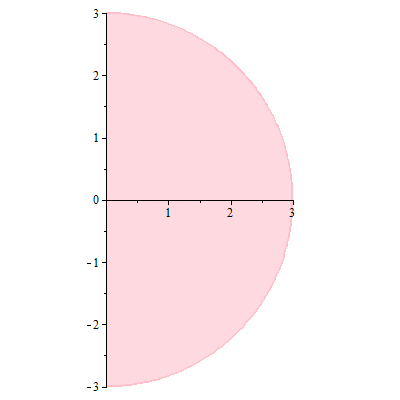
\includegraphics{11_4_Mass_exercise}}
  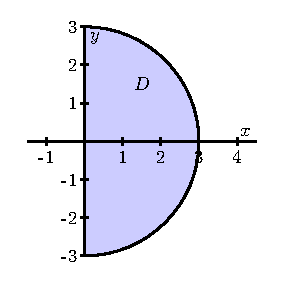
\includegraphics{figures/fig_11_4_half_circle.eps}
\end{center}
\caption{A half disk lamina.}
\label{F:11.4.Mass_exercise}
\end{figure}

\end{activity}
\begin{smallhint}

\end{smallhint}
\begin{bighint}

\end{bighint}
\begin{activitySolution}
We integrate the density over the region $D$. We have $\delta(x,y) = x$, and the region $D$ can be described by $0 \leq x \leq \sqrt{9-y^2}$ for $y$ between $-3$ and $3$. Thus, the mass of the lamina is
\begin{align*}
\int_{-3}^{3} \int_{0}^{\sqrt{9-y^2}} x \, dx \, dy &= \int_{-3}^{3} \left. \frac{x^2}{2} \right|_{0}^{\sqrt{9-y^2}} \, dy \\
	&= \int_{-3}^{3} \frac{1}{2}(9-y^2) \, dy \\
	&= \frac{1}{2} \left. \left[9y - \frac{1}{3}y^3\right]\right|_{-3}^{3} \\
	&= 18.
\end{align*}
\end{activitySolution}
\aftera
